\section{Design Thinking}\label{sec:08_04_Design_Thinking}
Beim Gestalten der Benutzeroberfläche haben wir uns an den sechs Phasen des von Tim Browns erfundenen Design Thinking Prozess orientiert. 

\begin{figure}[hbt!]
    \centering
    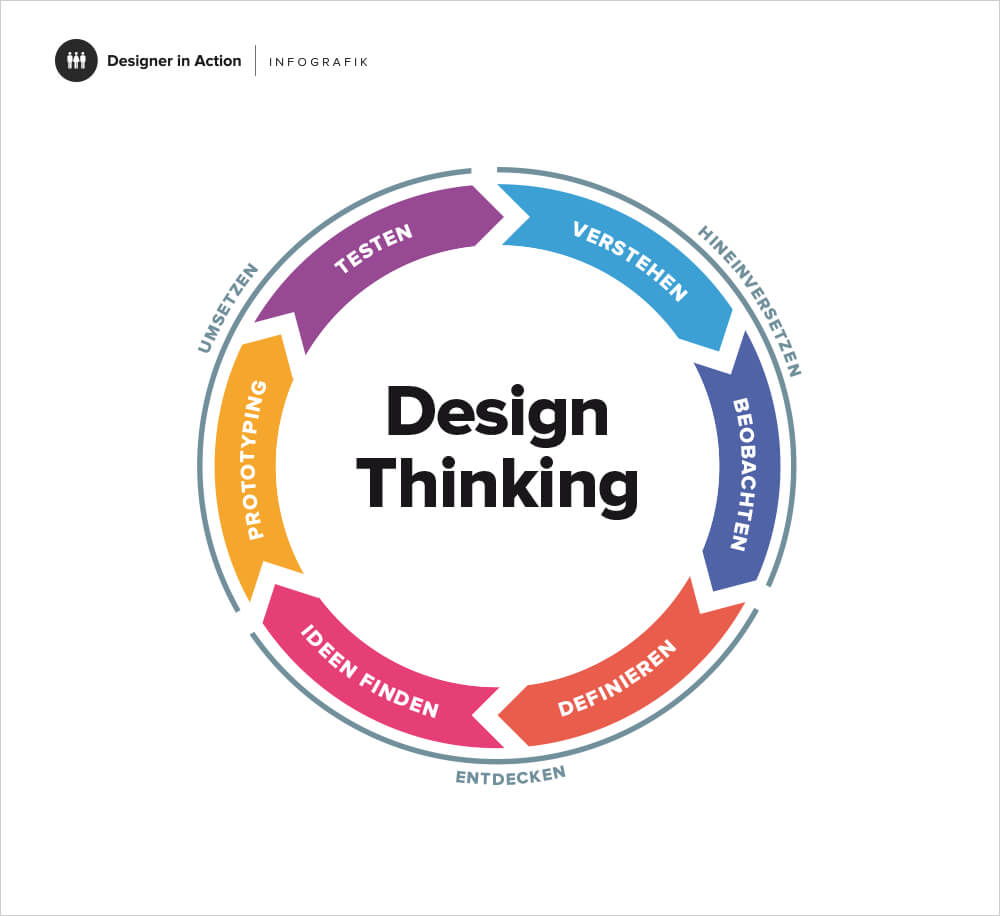
\includegraphics[width=14cm]{images/08-Benutzeroberfläche/08-Design Thinking.png}
    \caption{Ablauf des Design Thinking Prozess}
\end{figure}

Dieser Prozess wird im Online Artikel "Was ist Design Thinking?"\cite{DeTh} gut beschrieben. 
In diesem Projekt standen wir zunächst vor dem Problem, dass wir die Daten und fest definierten Schnittstellen erst im letzten drittel des Semesters vorliegen hatten. Vorher haben wir uns mit der Auswahl der Graphen- und Diagrammtypen beschäftigt. Wir haben Prototypen entwickelt und diese in regelmäßigen Abständen mit der Studentengruppe geteilt und Rückmeldungen gesammelt, welch in den Design Prozess eingeflossen sind. Mit den Rückmeldungen der Gruppe konnten wir unseren Prototypen verbessern, Teile umgestalten Beschreibungen anpassen oder Bereiche entfernen.
Die erste Iteration bestand in der Vorbereitung der Planungspräsentation unserer Gruppe. Bis zu diesem Zeitpunkt haben wir Ideen gesammelt, wie die angekündigten Daten in Diagrammen und für Benutzer*innen verständlich aufbereitet werden können. In einem Prototypen haben wir vier unterschiedliche Diagramme vorbereitet.

\begin{figure}[hbt!]%
    \centering
    \begin{subfigure}
        \centering
        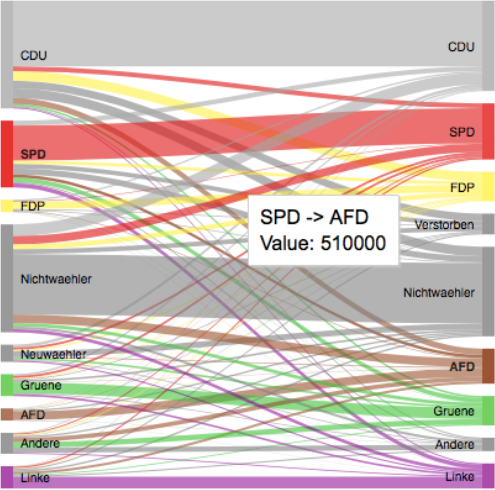
\includegraphics[width=5cm]{images/08-Benutzeroberfläche/08-flowchart.PNG}
    \end{subfigure}
    \qquad
    \begin{subfigure}
         \centering
         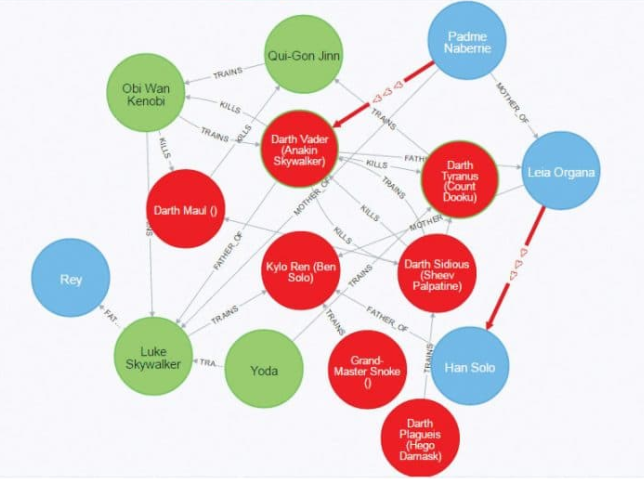
\includegraphics[width=5cm]{images/08-Benutzeroberfläche/08-Graphen.PNG}
    \end{subfigure}
    \qquad
    \begin{subfigure}
         \centering
        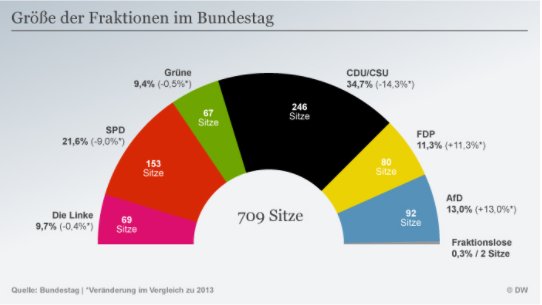
\includegraphics[width=5cm]{images/08-Benutzeroberfläche/08-Zusammensetzung_bundestag.PNG}
  \end{subfigure}
  \qquad
  \begin{subfigure}
        \centering
        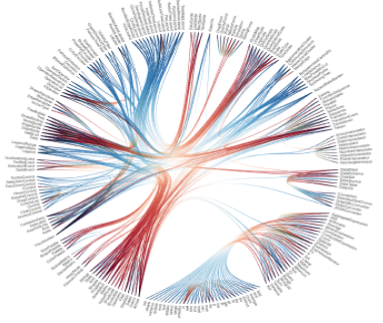
\includegraphics[width=5cm]{images/08-Benutzeroberfläche/08-Sehnendiagramm.PNG}
  \end{subfigure}
  \caption{Vorbereitete Diagramme der ersten Iteration}%
\end{figure}

Die Rückmeldungen und Diskussion am Ende der ersten Iteration, haben gezeigt, dass die direkte Visualisierung des Graphen zu unübersichtlich und nicht anschaulich ist. Ebenso ist das Sankey-Diagramm unübersichtlich und schwer zu interpretieren. Diese Diagramme sind nicht übernommen worden. Im Gegenteil dazu, wurden das Sehenendiagramm zur Visualisierung der Interaktionen und das halbe Kreisdiagramm zur Darstellung der Sitzeverteilung sehr positiv angenommen und deswegen weiter entwickelt.

In der zweiten Iteration wurden das Netzdiagramm und die Balkendiagramme integriert, die positives Feedback bekommen haben. Ebenfalls haben wir mit Box-Plots experimentiert, diese allerdings wegen der hohen Komplexität nicht weiter verfolgt.

\begin{figure}[hbt!]
    \centering
    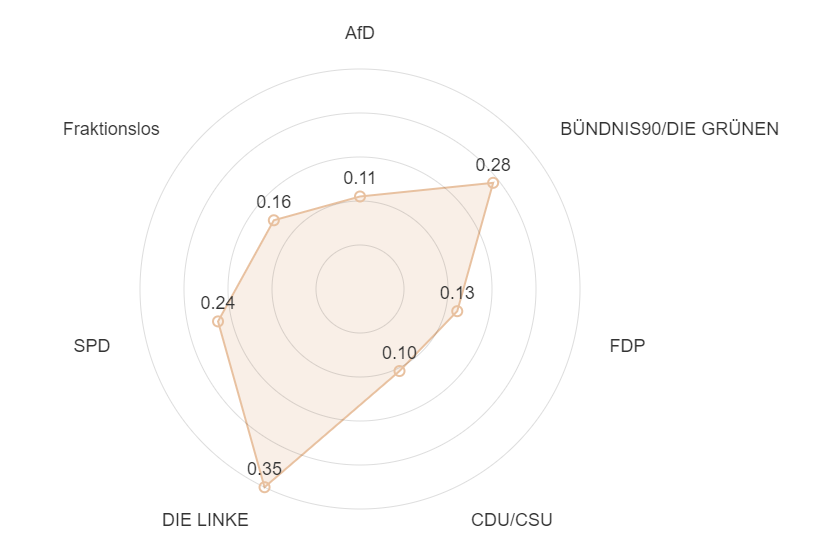
\includegraphics[width=8cm]{images/08-Benutzeroberfläche/08-Netzdiagramm.PNG}
    \caption{Eingeführtes Netzdiagramm}
\end{figure}

Nach den ersten beiden Iterationen standen die Diagrammtypen fest und wir konnten mit den einbetten der Diagramme in die Oberfläche beginnen. Dazu wurden die Diagramme in ein Storyboard eingebunden und mit Texten beschrieben. In den letzten Iterationen wurden Kleinigkeiten, wie die Texte und die Farben, abgestimmt um zum finalen Produkt zu gelangen.